\documentclass[10pt]{beamer}
% \documentclass[handout,10pt]{beamer}
\usepackage{my_style}

\title[Math/CS 375]{Lecture 15 - A}
\subtitle{\S 7.1, 7.2, 7.3 Euler's Method}

\begin{document}
% -------------------------------------------------
\begin{frame}
  \titlepage
\end{frame}
% -------------------------------------------------
\begin{frame}{Goals}
We will answer these questions:\\[3mm]
\begin{itemize}

    \item What are differential equations?
    
    \item In what way does a computer "solve" a differential equation?

    \item What is the difference between local and global error for ODE solvers?
    

\end{itemize}
\end{frame}

%%%%%%%%%%%%%%%%%%%%%%%%%%%%%%%%%
\sectionframe{Motivating Differential Equations}
%%%%%%%%%%%%%%%%%%%%%%%%%%%%%%%%%
\begin{frame}{Types of Equations to Solve}

\begin{block}{An Algebraic Equation}
Solve for \( x \in \mathbb{R} \) in:  
\[
x^2 - 2x - 8 = 0.
\]
\end{block}

\begin{block}{An Ordinary Differential Equation}
Solve for \( u(t) \in C^2(\mathbb{R}) \) in:  
\[
\frac{d^2 u}{dt^2} - 2\frac{du}{dt} - 8 = 0.
\]
The unknown $u$ is a function which depends on time.
\end{block}

\begin{block}{A Partial Differential Equation}
Solve for \( u(x, t) \in C^2(\mathbb{R} \times \mathbb{R})  \) in:  
\[
\frac{\partial^2 u}{\partial t^2} - \frac{\partial^2 u}{\partial x^2} = 0.
\]
\end{block}

\end{frame}

%%%%%%%%%%%%%%%%%%%%%%%%%%%%%%%%%

\begin{frame}{What is a Differential Equation?}

{\define{ODE}{
An \textbf{ordinary differential equation} is an equation that relates a function \( u(t) \) to its derivatives:
\[
F\left(t, u, u', u'', \dots\right) = 0.
\]
}}

\vspace{3mm}

\begin{block}{Examples}
\begin{itemize}
    \item First-order: \( u' + u = 0 \)
    \item Second-order: \( u'' - 3u' + u = 0 \)
    \item Nonlinear: \( u' - u^2 - t  = 0\)
\end{itemize}
\end{block}

\vspace{3mm}

\begin{block}{Why study DEs?}
    \begin{itemize}
        \item Used to model systems that change over time or space
        \item Physics, biology, engineering, economics
    \end{itemize}
\end{block}

\end{frame}
%%%%%%%%%%%%%%%%%%%%%%%%%%%%%%%%%
\begin{frame}{Example: Snowball Effect}{Model}

\begin{block}{Problem}
Suppose a snowball with an initial radius $r=1$ is rolled down from the top of a snowy mountain. Find an equation for the radius of the snowball at time $t$.  
\end{block}

\begin{itemize}
    \item This is a difficult problem
    \item The goal is to derive $r(t) = $ the radius of the snowball at time $t$
    \item We need to make simplifying assumptions
\end{itemize}

{
\question{How should the radius change over time? What influences the growth rate? How do differential equations come into play?}
}
% \begin{figure}
%     \centering
%     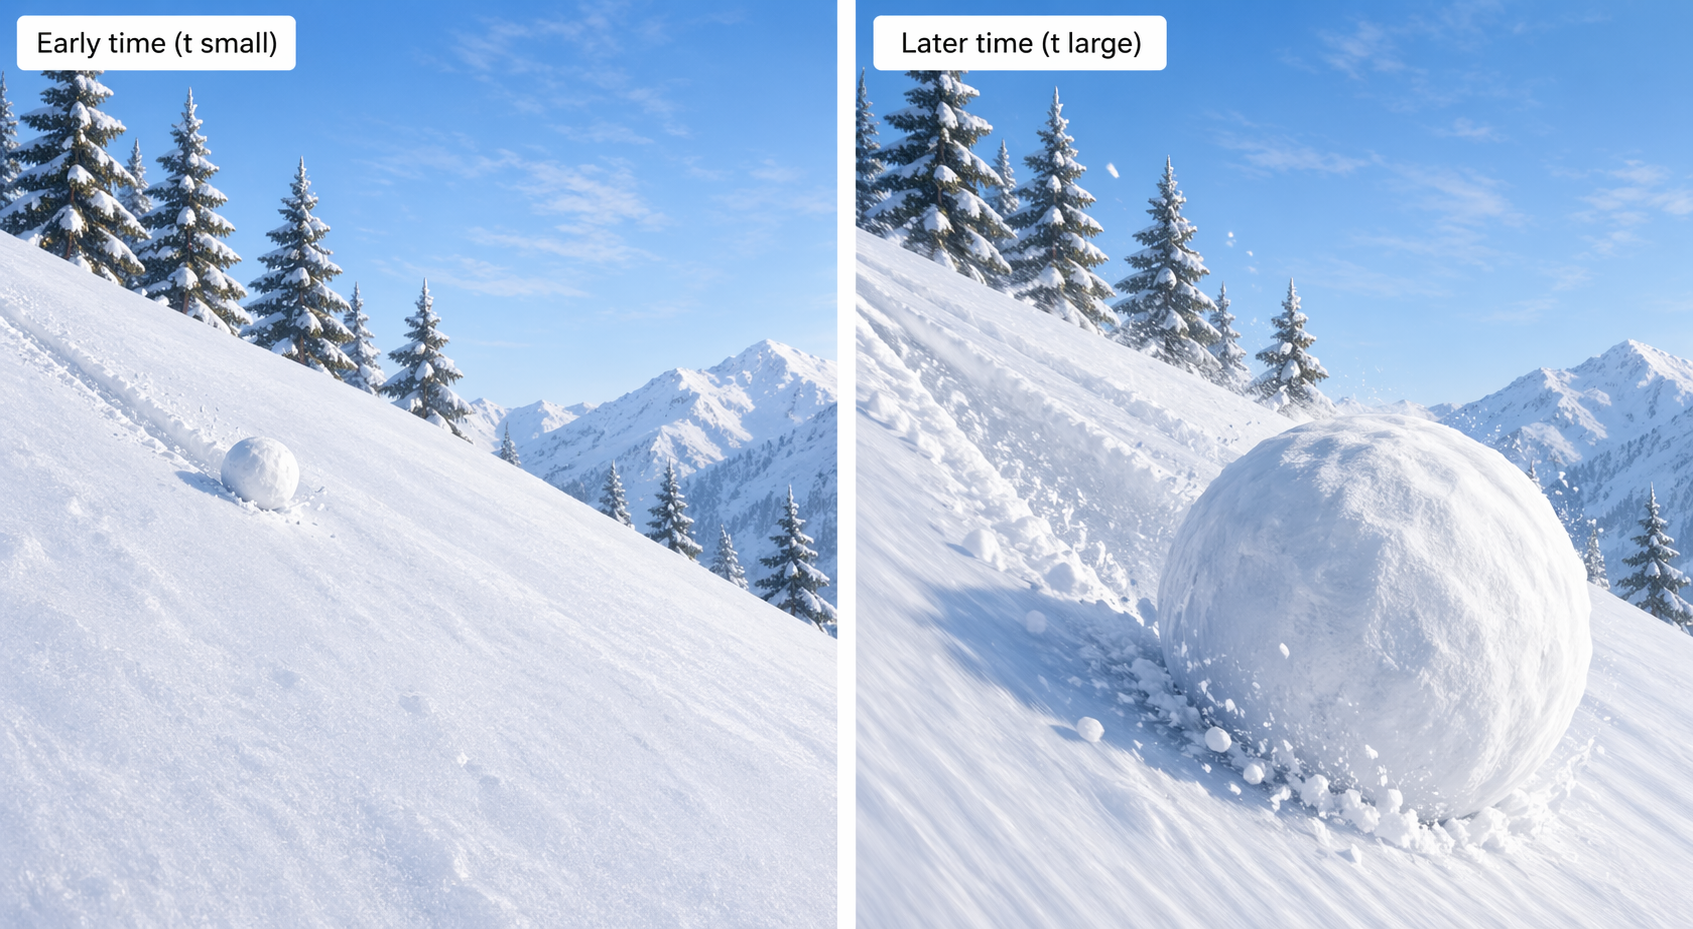
\includegraphics[width=0.8\linewidth]{figs/snowball.png}
% \end{figure}
\end{frame}
%%%%%%%%%%%%%%%%%%%%%%%%%%%%%%%%%
\begin{frame}{Example: Snowball Effect}{Assumptions}
\begin{figure}
    \centering
    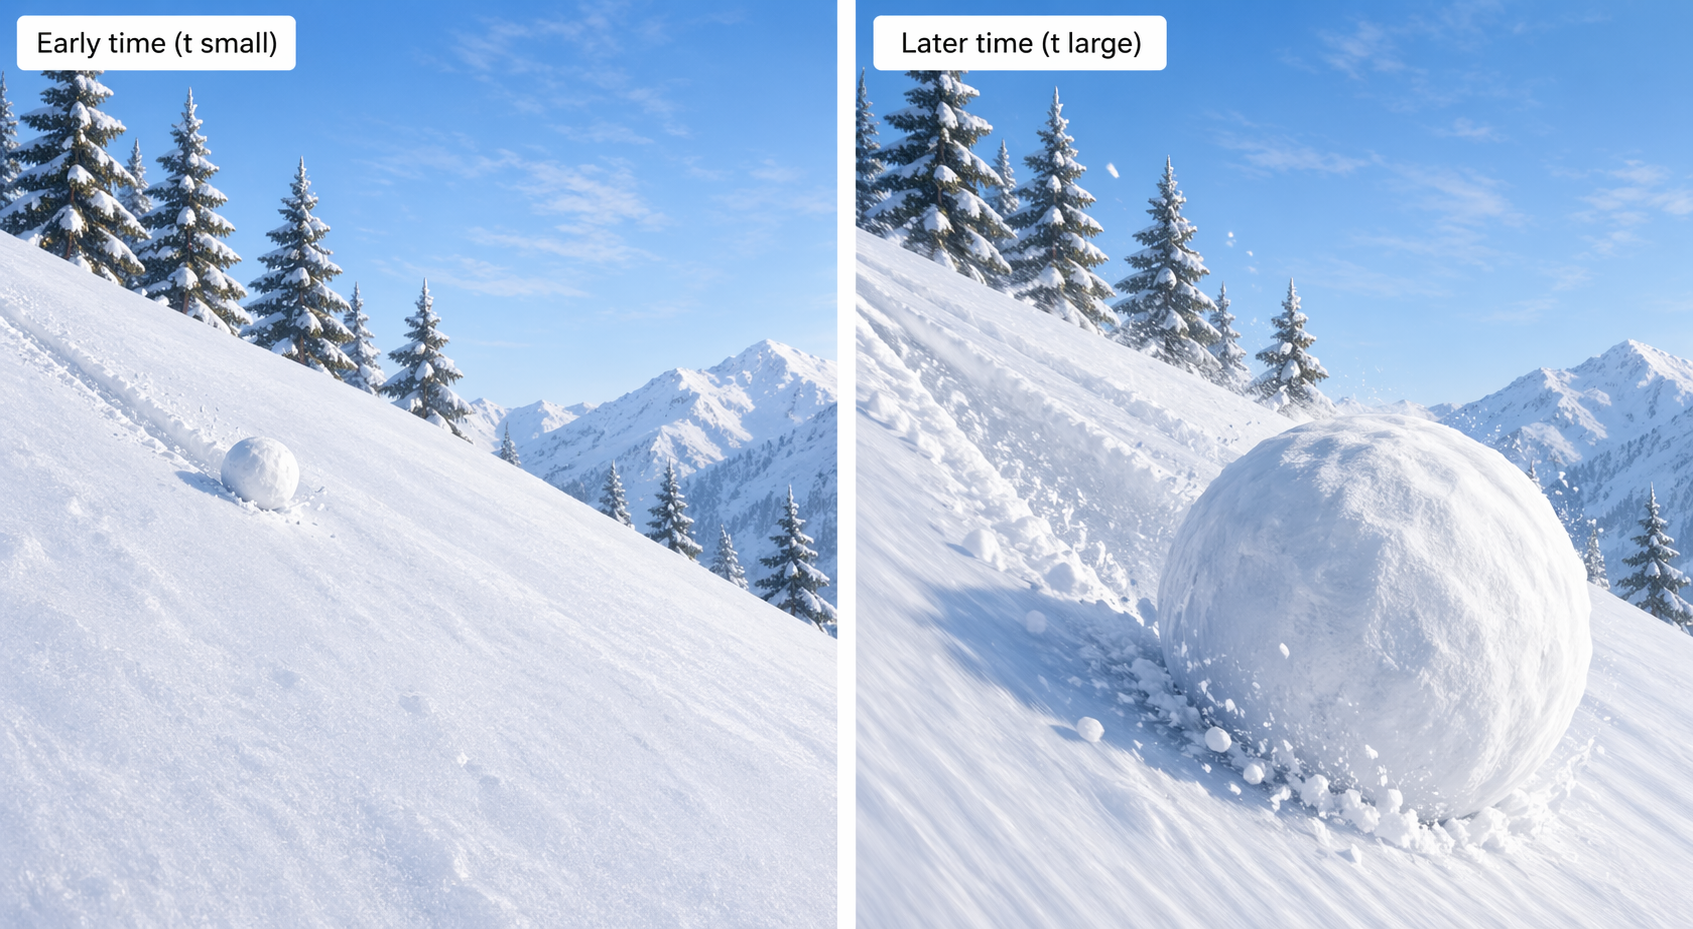
\includegraphics[width=0.8\linewidth]{figs/snowball.png}
\end{figure}
\begin{itemize}
    \item As a simple model, assume the radius grows at a rate proportional to the radius 
    \item smaller snowball $\implies$ slower growth
    \item bigger snowball $\implies$ faster growth
\end{itemize}



\end{frame}
%%%%%%%%%%%%%%%%%%%%%%%%%%%%%%%%%

\begin{frame}{Example: Snowball Effect}{Model}

\begin{itemize}
    \begin{block}{Model for the Snowball}       
    Let $r(t)$ be the radius at time $t$  
        \begin{equation*}
            \underbrace{\frac{dr}{dt}}_{\textrm{growth speed}} = k\underbrace{r}_{\textrm{current size}} 
        \end{equation*}
    Constant $k>0$ is a proportionality constant.
    \end{block}
    \item If $r$ is small, $r'$ is small
    \item If $r$ is large, $r'$ is large
\end{itemize}

{
\define{Model}{ A \textbf{mathematical model} uses mathematical relationships to describe a system; here we use a differential equation. }
}
\end{frame}
%%%%%%%%%%%%%%%%%%%%%%%%%%%%%%%%%%%%%%%%%%%%
\begin{frame}{Example: Snowball Effect}{Solution}

\begin{itemize}
    \item We let $t=0$ be the time when the snowball begins to roll 
    \item Since the initial radius is 1, we write $r(0) = 1$ 

    \item The full problem is to solve for the function $r(t)$ in
        $$\begin{dcases}
        \frac{dr}{dt} = kr,  & t>0\\
           r(0) = 1 &
        \end{dcases}$$
    
    \begin{block}{Solution}
    The exact solution is 
        $$r(t) = e^{kt} $$
    The size of the snowball grows exponentially with rate $k$.
    \end{block}
        \vspace{3mm}
    \item \textit{The focus of this class is to not solve DEs by hand, but numerically.}
\end{itemize}
\end{frame}



%%%%%%%%%%%%%%%%%%%%%%%%%%%%%%%%%%%%%%%%%
\begin{frame}{Main Idea}

\begin{block}{1. Difficult Problem}
    Find the equation for the size of the snowball.
\end{block}

\begin{block}{2. Simplifying Assumption}
    Snowball's size increases proportional to its current size.
\end{block}

\begin{block}{3. Differential Equation}
    $$r' = kr$$
\end{block}

\begin{block}{4. Solution}
Radius of the snowball as a function of time
    $$r(t) = e^{kt}$$
\end{block}
\end{frame}



%%%%%%%%%%%%%%%%%%%%%%%%%%%%%%%%%%%%%%%%%
\sectionframe{Initial Value Problems}

\begin{frame}{}
    \begin{itemize}
        \item The model for the size of the snowball is
                $$\begin{dcases}
                r' = kr,  & t>0\\
           r(0) = 1 &
        \end{dcases}$$
        \item The equation $r'=kr$ is the \textbf{differential equation}
            \vfill 
        \item The equation $r(0)=1$ is called the \textbf{initial condition}
            \vfill  

        \item A differential equation together with an initial condition is called an \textit{initial value problem}
            \vfill  
    \end{itemize}
\end{frame}

\begin{frame}{Initial Value Problems (IVPs)}
   
\define{IVP}{
    An \textbf{initial value problem} is the task to solve the time-dependent function $u(t)$ given a differential equation and an initial condition. 
    $$\begin{dcases}
    F\left(t, u, u', \dots\right) = 0,  & t>0\\
       u(0), u'(0), \dots \text{given}, & t=0
    \end{dcases}$$
}

Examples:
\begin{enumerate}
\item First order IVP

\begin{align*}
\begin{cases}
u^\prime = f(t,u(t)), \quad t \in (0,T]\\
u(0) = u_0
\end{cases}
\end{align*}

\item Second order IVP
\begin{align*}
\begin{cases}
m u^{''}(t) + c u^\prime (t) + k u (t) = f(t), \quad t \in (0,T]\\
u(0) = A, u^\prime(0) = B
\end{cases}
\end{align*}

\end{enumerate}

\end{frame}

%%%%%%%%%%%%%%%%%%%%%%%%%%%%%%%%%%%%%%%%%%
\begin{frame}{Second Order Example}


\cols{

\begin{block}{Problem}
    Suppose a rock with mass $m$ is dropped from a cliff that is 50 meters high. What is the elevation of the rock as a function of time after its release?
\end{block}



\begin{block}{Assumption}
\begin{itemize}
    \item No wind resistance
    \item Constant gravity; model valid until impact
    \item Use Newton's Law $F=ma=-mg$
\end{itemize}
\end{block}
% \begin{block}{Model}
% Let $x(t)=$ elevation of the rock (up is positive).
% \begin{align*}
% \begin{cases}
% x^{''} = -g, \quad t \in (0,T]\\
% x(0) = 50,\; x^\prime(0) = 0
% \end{cases}
% \end{align*}
% \end{block}

}{
\begin{figure}
    \centering
    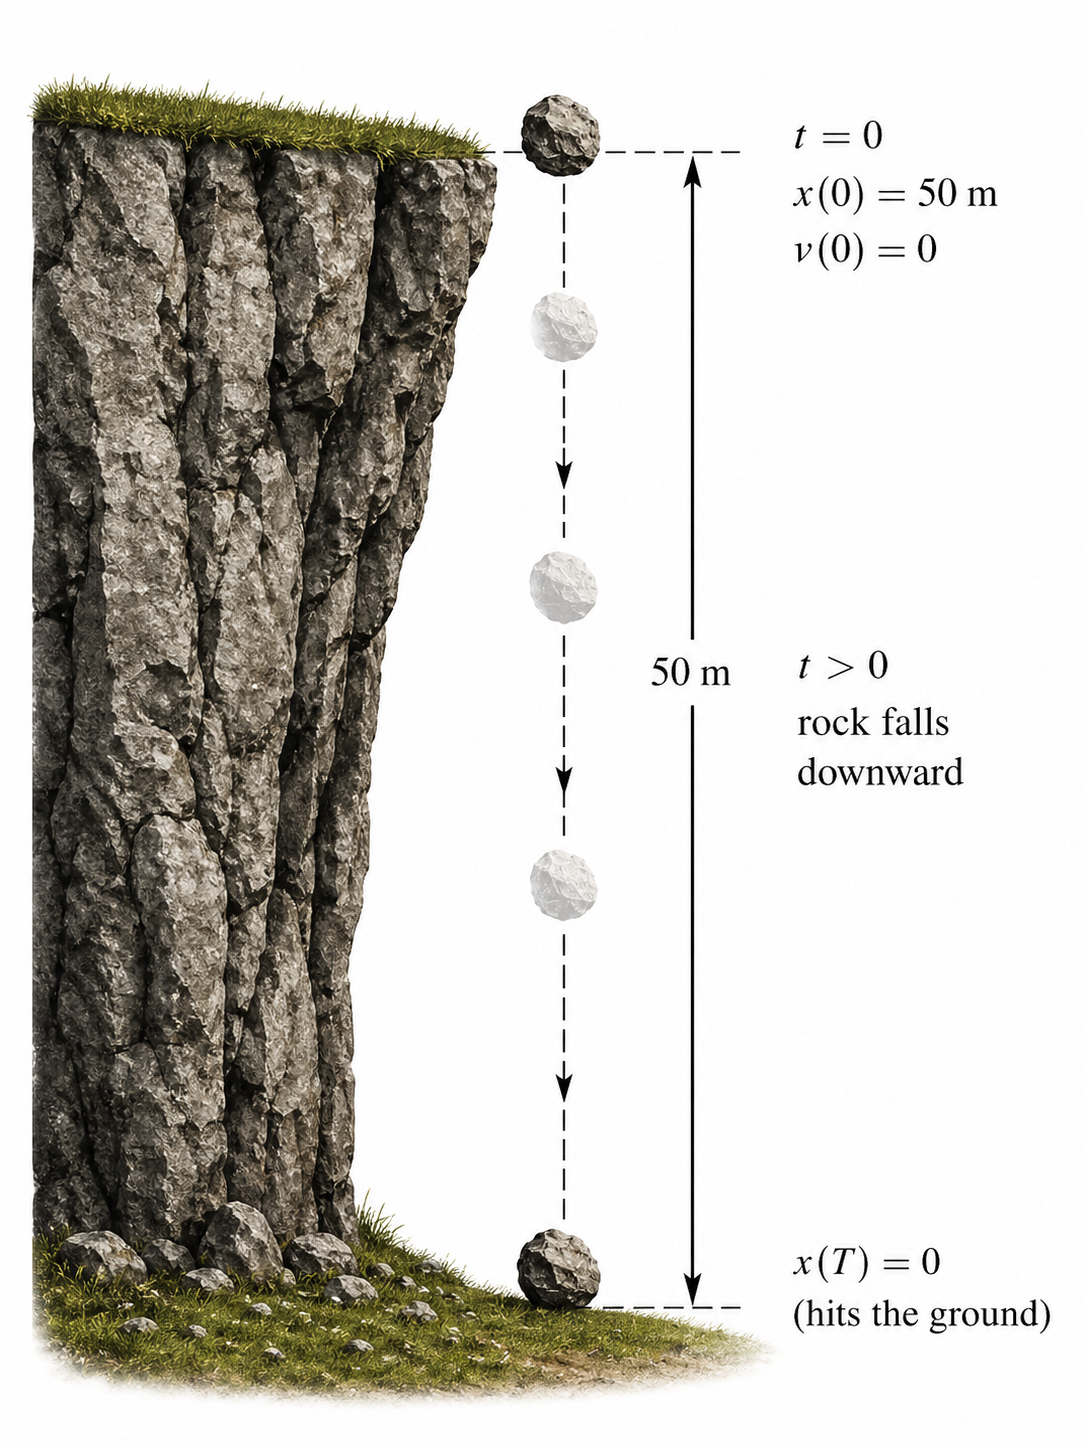
\includegraphics[width=0.9\linewidth]{figs/cliff.png}
\end{figure}
}

\end{frame}

%%%%%%%%%%%%%%%%%%%%%%%%%%%%%%%%%%%%%%%%%%
\begin{frame}{Second Order Example}


\cols{
\begin{itemize}
    \item  Let $x(t)=$ elevation of the rock (up is positive).

\end{itemize}
\begin{block}{Model}
\begin{align*}
\begin{cases}
x^{''} = -g, \quad t \in (0,T]\\
x(0) = 50,\; x^\prime(0) = 0
\end{cases}
\end{align*}
\end{block}

\begin{block}{Solution}
\begin{align*}
x(t) = 50 - \frac{1}{2}gt^2
\end{align*}
\end{block}

}{
\begin{figure}
    \centering
    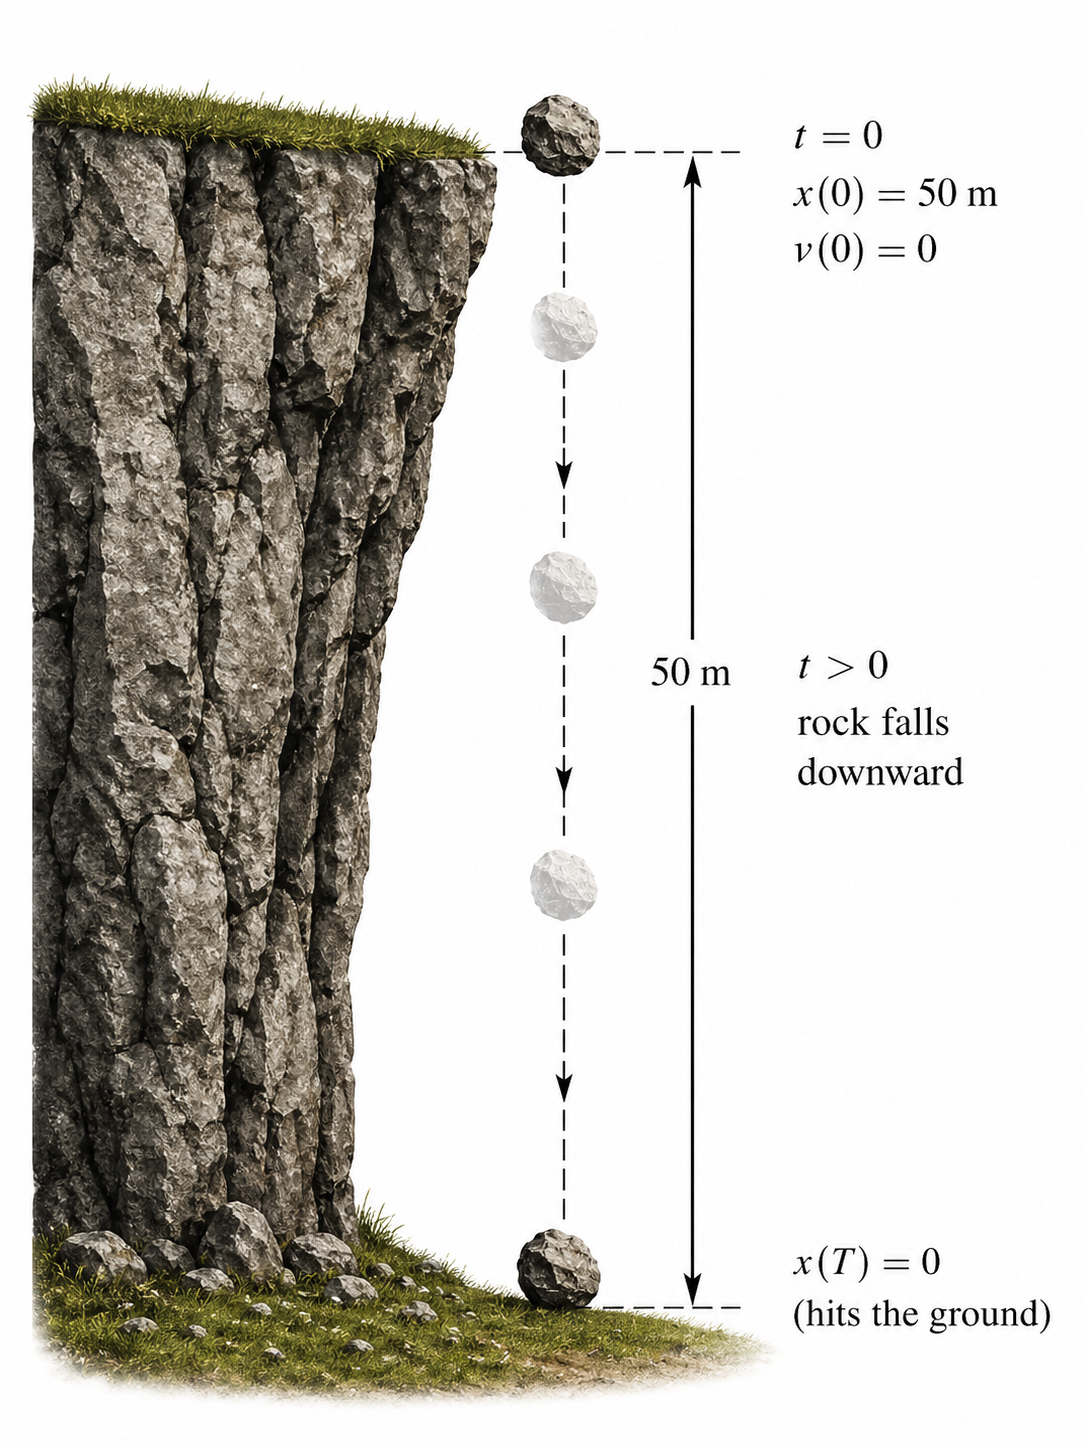
\includegraphics[width=0.9\linewidth]{figs/cliff.png}
\end{figure}
}

\end{frame}
%%%%%%%%%%%%%%%%%%%%%%%%%%%%%%%%%%%%%%%%%%
\begin{frame}{Verifying a Solution}

\question{
If you were given the solution $u(t)$ to an IVP, how do you mathematically verify that it truly is a solution?
}
\vfill
\textbf{Steps:}
\begin{itemize}
    \item First, substitute $u(t)$ into the left-hand side (LHS) of the DE
    \item Next, substitute $u(t)$ into the right-hand side (RHS) of the DE
    \item Show that LHS = RHS 
    \item Verify that the initial condition holds
\end{itemize}

    
\end{frame}

%%%%%%%%%%%%%%%%%%%%%%%%%%%%%%%%%%%%%%%%%%
\begin{frame}{Verifying a Solution 1}
\begin{example}
    Show that $r(t)=e^{kt}$ solves the IVP
    $$\begin{dcases}
        \frac{dr}{dt} = kr  & t>0\\
           r(0) = 1 & 
    \end{dcases}$$
\end{example}
\begin{itemize}
    \item LHS is 
    \begin{align*}
        \text{LHS} &= \frac{dr}{dt} =(e^{kt})'= ke^{kt}
    \end{align*}
    \item The RHS is 
    \begin{align*}
        \text{RHS} &= kr= k(e^{kt})=\text{LHS}
    \end{align*}
    \item Then verify the initial condition $r(0) = e^{k0}=e^{0}=1.$
\end{itemize}
    
\end{frame}

%%%%%%%%%%%%%%%%%%%%%%%%%%%%%%%%%%%%%%%%%%
\begin{frame}{Verifying a Solution 2}
\begin{example}
    Show that $x(t) = 50 - \frac{1}{2}gt^2$ solves the IVP
    $$\begin{cases}
x^{''} = -g, \quad t \in (0,T]\\
x(0) = 50,\; x^\prime(0) = 0
\end{cases}$$
\end{example}
\begin{itemize}
    \item LHS is 
    \begin{align*}
        \text{LHS} &= x'' =(50 - \frac{1}{2}gt^2)''= -g
    \end{align*}
    \item The RHS is 
    \begin{align*}
        \text{RHS} &=-g = \text{LHS}
    \end{align*}
    \item Then verify the initial conditions $x(0) = 50$ and $x'(0)=0.$ 
\end{itemize}
    
\end{frame}

\begin{frame}{First-Order IVP}
    \begin{block}{First-Order IVP}
        Given a rate law $f(t,u)$ and an initial value, find a function $u(t)$ satisfying both: 
        $$
        \begin{cases}
		u^\prime = f(t,u(t)), \quad t \in (a,b]\\
		u(a) = u_a
	\end{cases}
        $$
    \end{block}

    \begin{theorem}
        If $f = f(t,u)$ and $\partial f/\partial u$ are continuous in the rectangle $\{ |t-a|<\alpha , \; |u-u_a|<\beta  \}$, then the first-order IVP has a unique continuously differentiable solution in some interval $|t-a| < \epsilon$.  
    \end{theorem}

\end{frame}



%%%%%%%%%%%%%%%%%%%%%%%%%%%%%%%%%%%%%%%%%%%%
\sectionframe{Time-Stepping Algorithms}
%%%%%%%%%%%%%%%%%%%%%%%%%%%%%%%%%%%%%%%%%%%%

\begin{frame}{Analytic and Numerical Solutions}
\begin{block}{Examples with analytic solutions}
\begin{itemize}
    \item $x' = xt$
    \item $x''+4x'+2x=0$
    \item $t^2x'' + tx'+x=0 $
\end{itemize}
\end{block}

\begin{block}{Often approached numerically}
\begin{itemize}
    \item $x'=\cos(xt)$
    \item $x'' + x^2x' +x=0 $
    \item $x'' + \sin(x') +x^3=\cos t$
\end{itemize}
\end{block}
\begin{center}
    Only a small class of DEs can be solved by hand.
\end{center}
\end{frame}

%%%%%%%%%%%%%%%%%%%%%%%%%%%%%%%%%%%%%%%%%%%%

\begin{frame}{Numerical Solution of IVPs}

\begin{block}{The need for approximations}
\begin{itemize}
    \item Many important ODEs have \underline{no closed-form solution}
    \item We can only solve a few types of ODEs by hand
\end{itemize}    
\end{block}
    \vspace{5mm}

    \question{
        What does it mean to solve for the solution $u(t)$ on the computer?
    }
\end{frame}


%%%%%%%%%%%%%%%%%%%%%%%%%%%%%%%%%%%%%%%%%%%%
\begin{frame}{Numerical Solution of IVPs}

    \begin{figure}
        \centering
        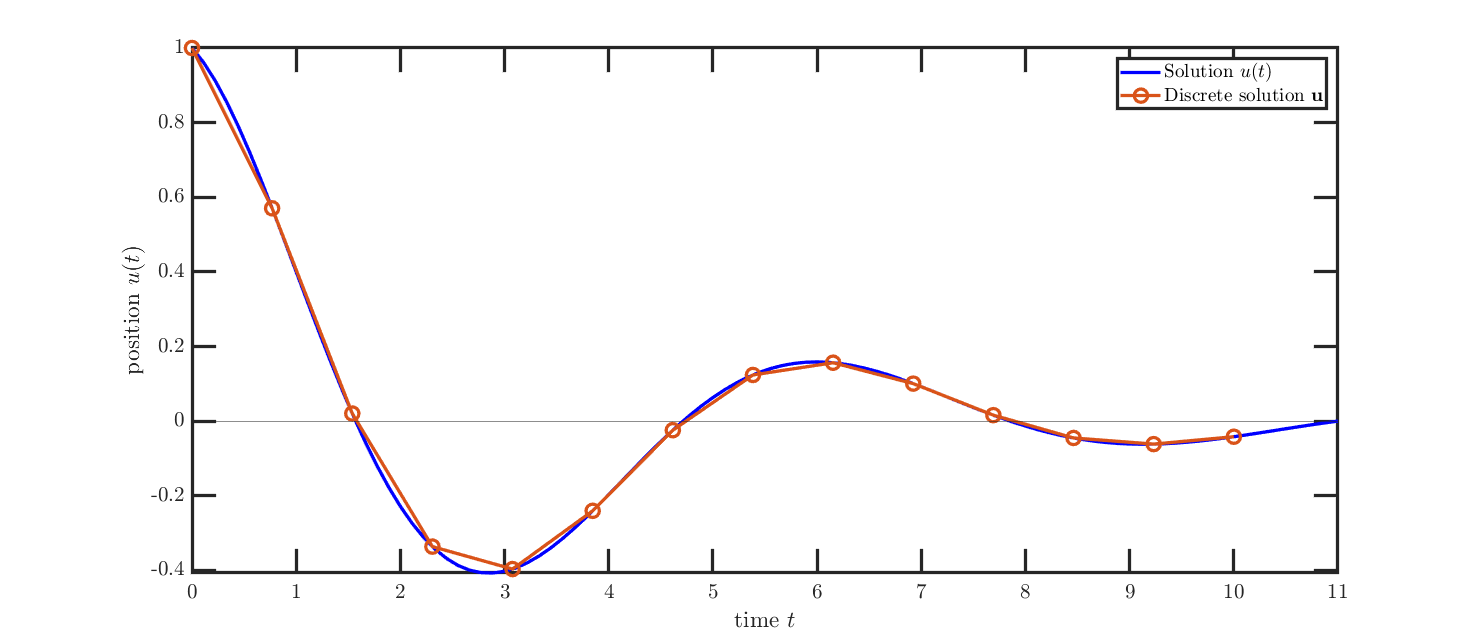
\includegraphics[scale=0.3]{figs/discrete_ODE.png}\\
    \end{figure}
    

    \begin{itemize}
        \item Numerical ODE solvers approximate values at selected times
        \item They find a discrete approximation $\textbf{u}$ of the continuous $u(t)$ 
    \end{itemize}    

\keyidea{
We replace a continuous function with values at discrete time steps.
}
\end{frame}


%%%%%%%%%%%%%%%%%%%%%%%%%%%%%%%%%%%%%%%%%%%%
\begin{frame}{The Problem}

    \begin{block}{First-Order Initial Value Problem}
        
    Consider the task of solving for the unknown function $u(t)$ in:
        $$
        \begin{cases}
		u^\prime = f(t,u(t)), \quad t \in (a,b]\\
		u(a) = u_a
	\end{cases}
        $$
    \end{block}

    \begin{block}{Solution}
    Assume the solution $u(t)$ exists throughout $[a,b]$.
    \end{block}

    \begin{block}{Objective}
    Since we cannot find $u(t)$ in general, our goal is to find a \textit{discrete approximation} to $u$.
    \end{block}
\end{frame}

%%%%%%%%%%%%%%%%%%%%%%%%%%%%%%%%%%%%%%%%%%%%
\begin{frame}{The Discrete Solution}
\begin{itemize}
    \item Discretize $[a,b]$ into equi-spaced points:
	\[a = t_0 < t_1 < t_2 < \cdots < t_{n-1} < t_n = b\]
	with $h = t_{i} - t_{i-1} = (b-a)/n$
    \item Our discrete numerical solution is 
    \begin{equation*}
        \textbf{u} = \begin{bmatrix} \textbf{u}_0 \\ \textbf{u}_1 \\ \vdots \\  \textbf{u}_n \end{bmatrix} \approx  \begin{bmatrix} u(t_0) \\ u(t_0 + h) \\ \vdots \\  u(t_0 + nh) \end{bmatrix}
    \end{equation*}
    \item Initial condition is given: $\textbf{u}_0 = u(t_0)$ 
    \item We want an algorithm to produce 
    $$
    \textbf{u}_i \approx u(t_0 + ih)
    $$
    for $i=1,\ldots, n$
\end{itemize}
\end{frame}
%%%%%%%%%%%%%%%%%%%%%%%%%%%%%%%%%%%%%%%%%%%%
\begin{frame}{Time-Stepping Algorithms}
    \begin{block}{Goal}
        Construct the vector $\textbf{u}$ whose elements are $\textbf{u}_i \approx u(t_0 + ih)$. 
    \end{block}

    \vspace{3mm}

    {\question{
        If you know $\textbf{u}_0$, how would you approximate the solution at the next time step $\textbf{u}_1$?
    }}
    

    \begin{block}{Main Idea: Use recursion}
    
    \begin{itemize}
        \item Suppose you have an update formula $$\textbf{u}_{i+1} = T(t_{i},\textbf{u}_{i};h)$$ where $T()$ is the update function\\[3mm]
        \item We can recursively find all values of $\textbf{u}_i$
        \item This is the main idea of \textbf{Time-Stepping algorithms}
    \end{itemize}
    \end{block}
\end{frame}

%%%%%%%%%%%%%%%%%%%%%%%%%%%%%%%%%%%%%%%%%%%%
\begin{frame}{Time-Stepping Algorithms}
    \begin{block}{Goal}
        Construct the vector $\textbf{u}$ whose elements are $\textbf{u}_i \approx u(t_0 + ih)$. 
    \end{block}

    \vspace{2mm}
    \textbf{Assume you know}:
    \begin{itemize}
        \item Initial condition $\textbf{u}_0$
        \item Update function $T$ satisfying
        $$\textbf{u}_{i+1}  =   T(t_{i},\textbf{u}_{i};h)$$
    \end{itemize}
    
    \textbf{Do a time-stepping loop}:
        \begin{align*}
            \textbf{u}_1 &=  T(t_{0},\textbf{u}_{0};h) \\ 
            \textbf{u}_2 &= T(t_{1},\textbf{u}_{1};h) \\
                        &\vdots \\
            \textbf{u}_n &= T(t_{n-1},\textbf{u}_{n-1};h) 
        \end{align*}

\end{frame}

%%%%%%%%%%%%%%%%%%%%%%%%%%%%%%%%%%%%%%%%%%%%
\begin{frame}[fragile]{Time Stepping Pseudocode}

\begin{itemize}
    \item In general the update function $T$ may depend on $u$ and $t$, 
        $$T = T(t,u;h)$$

    \item Start by initializing an empty vector for the solution 
    \item Create a discretization of time 
    \item View time-stepping as an iterative method
\end{itemize}
\begin{lstlisting}[mathescape,label=algo,caption=Simple Time-stepping]
u = zeros(n+1,1)
t = linspace(a,b,n+1)
h = (b-a)/n
u(1) = $u_0$ % given data
for i = 1 : n 
    u(i+1) = $T$(t(i),u(i),h)
end
\end{lstlisting}
\end{frame}

%%%%%%%%%%%%%%%%%%%%%%%%%%%%%%%%%%%%%%%%%%%%
\sectionframe{Euler's Method}
%%%%%%%%%%%%%%%%%%%%%%%%%%%%%%%%%%%%%%%%%%%%

\begin{frame}{Use Taylor Expansion}{Part 1}

\begin{block}{Goal}
    Come up with formula for $\textbf{u}_{i+1}$ which depends on $\textbf{u}_i$. 
\end{block}

\begin{itemize}
    \item Taylor's Expansion of $u(t_i+h)$
    \begin{align*}        
    u(t_i+h) &= u(t_i) + h u^\prime(t_i) + (h^2/2) u^{''}(c), \quad t_i < c < t_i+h\\
           &\approx u(t_i) + h u'(t_i) 
    \end{align*}

    \item Recall that we are trying to solve the first order IVP 
        $$
        \begin{cases}
		u^\prime = f(t,u(t)), \quad t \in (a,b]\\
		u(a) = u_a
	\end{cases}
        $$
    \item We can substitute $u'(t_i) = f(t_i, u(t_i))$
\end{itemize}

\end{frame}
%%%%%%%%%%%%%%%%%%%%%%%%%%%%%%%%%%%%%%%%%%%%
\begin{frame}{Use Taylor Expansion}{Part 2}

\begin{block}{Goal}
    Come up with formula for $\textbf{u}_{i+1}$ which depends on $\textbf{u}_i$. 
\end{block}

\begin{itemize}
    \item Taylor's Expansion of $u(t_i+h)$ with $f$
    \begin{align*}        
    u(t_i+h) &= u(t_i) + h u^\prime(t_i) + (h^2/2) u^{''}(c), \quad t_i < c < t_i+h\\
           &\approx u(t_i) + h u'(t_i) \\
           &= u(t_i) + h f(t_i, u(t_i))
    \end{align*}

    \item Now use the discrete approximation $\textbf{u}_i \approx u(t_i)$
        $$
        \textbf{u}_{i+1} = \textbf{u}_i + h\,f(t_i, \textbf{u}_i )
        $$
    \item This is called \textbf{Euler's Method}.
\end{itemize}

\end{frame}
%%%%%%%%%%%%%%%%%%%%%%%%%%%%%%%%%%%%%%%%%%%%
\begin{frame}[fragile]{Euler's method}

\method{Euler's Method}
{ODE $u'=f(t,u)$, initial condition $u_0$}
{Discrete approximation to $u(t)$}
{Use the approximation $u(t+h)\approx u(t) + h f(t,u(t))$}

\begin{itemize}
    \item Euler's method is given by the recurrence equation 
        $$
        \textbf{u}_{i+1} = \textbf{u}_i + h\,f(t_i, \textbf{u}_i )
        $$
    \item Very simple code
\end{itemize}
\begin{lstlisting}[mathescape,label=algo]
u(1) = $u_a$
for i = 1 : n
    u(i+1) = u(i) + h * f(t(i),u(i))
end
\end{lstlisting}
\end{frame}

%%%%%%%%%%%%%%%%%%%%%%%%%%%%%%%%%%%%%%%%%%%%
\begin{frame}{Euler Example}{(Not to be done by hand)}
\begin{example}
Apply Euler's method with $h = 0.2$ to the IVP
\[
\begin{cases}
u^\prime = tu + t^3, \qquad t \in [0,1]\\
u(0) = 1
\end{cases}
\]
\end{example}
\begin{itemize}
    \item $h = (b-a)/n \, \,\implies n = 5$
\begin{center}
\begin{tabular}{c|l|l|l}
 $i$ & $t_i$ & $\textbf{u}_i$ & $f(t_i,\textbf{u}_i) = t_i \textbf{u}_i + t_i^3$  \\ \hline 
 0& 0.0& 1.0&           0.0 \\
 1& 0.2& 1.0&    0.2080\\
 2& 0.4& 1.0416& 0.4806\\
 3& 0.6& 1.1377& 0.8986\\
 4& 0.8& 1.3175& 1.5660\\
 5& 1.0& 1.6306&       \\
\end{tabular}
\end{center}\bigskip
\item The column $u_i$ is the numerical solution
\end{itemize}
\end{frame}
%%%%%%%%%%%%%%%%%%%%%%%%%%%%%%%%%%%%%%%%%%%%
\begin{frame}{Euler Example}
\begin{itemize}
    \item Exact solution is 
    \[
    u(t) = 3 e^{t^2/2} - t^2 - 2
    \]
    \item Euler's method with $h = 0.2, 0.1, 0.05$
    \begin{equation*}
      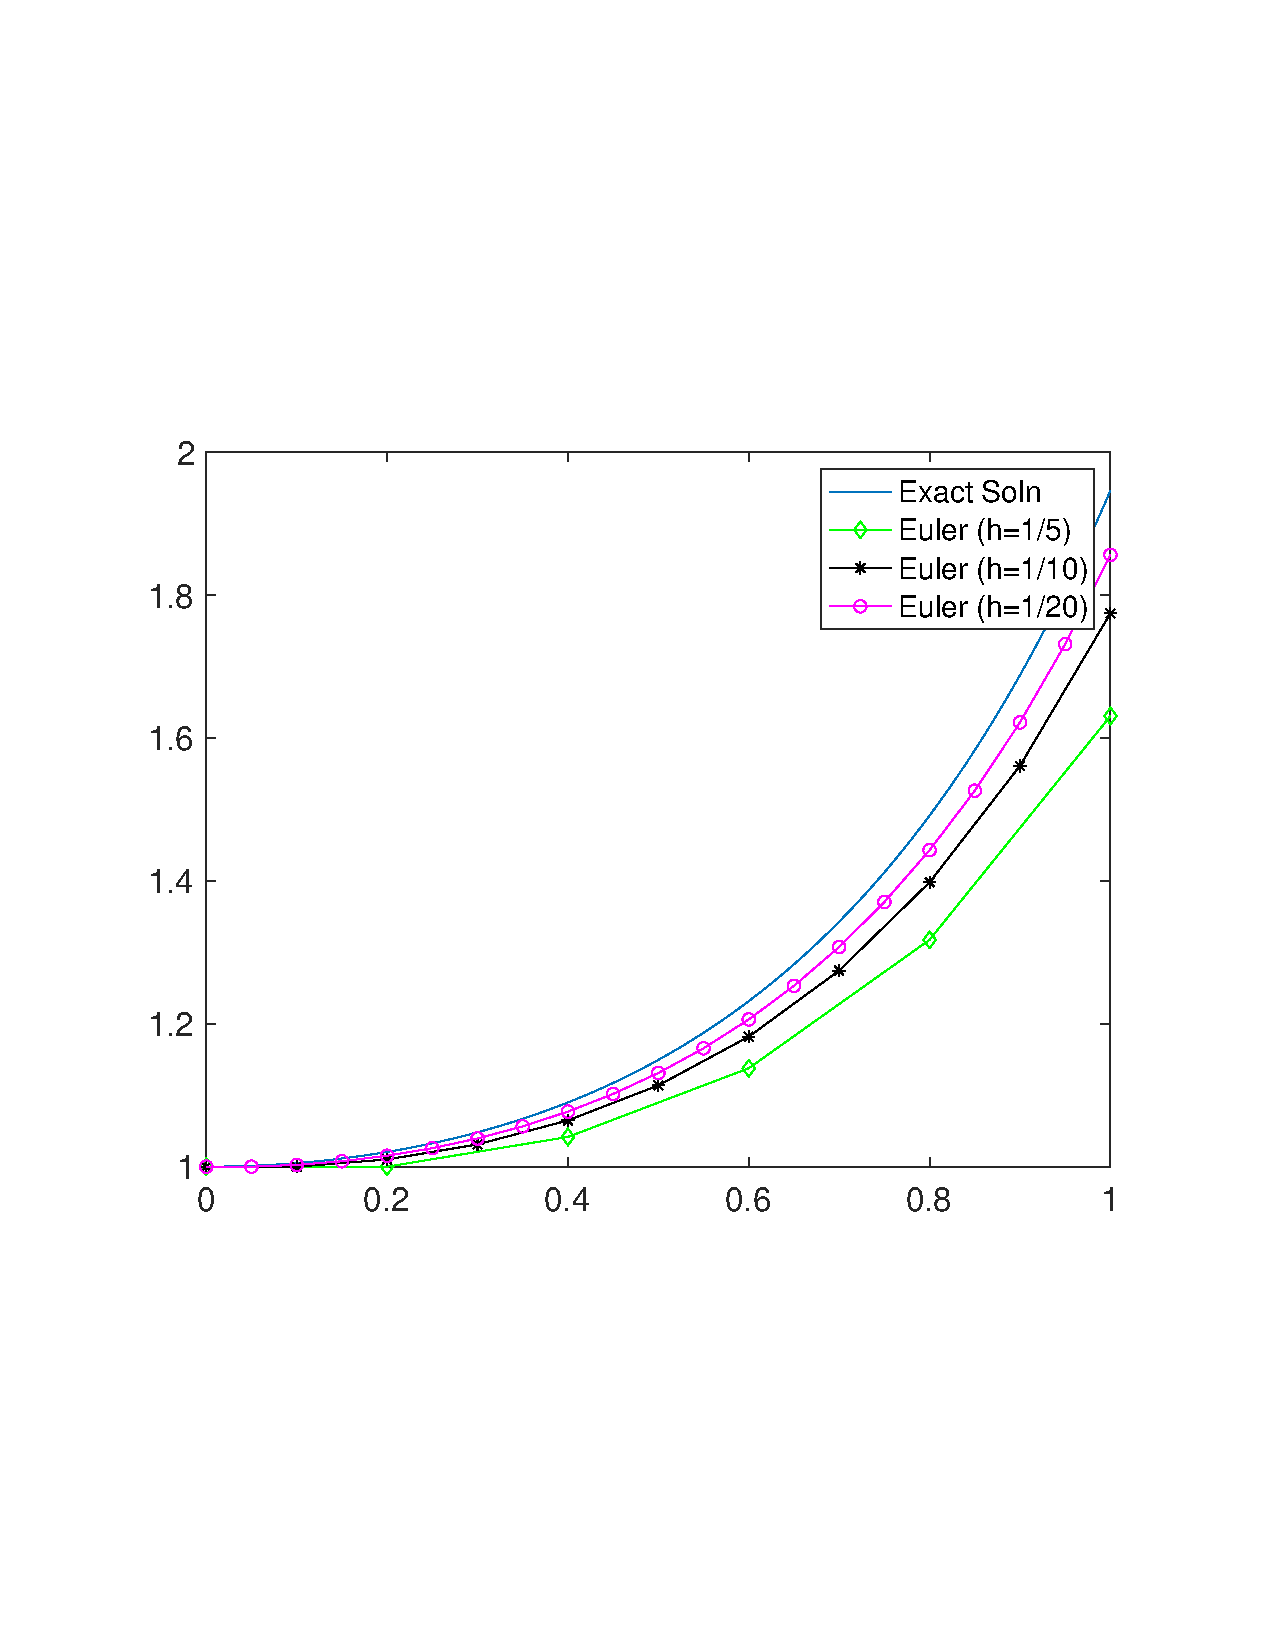
\includegraphics[height=5cm]{./figs/for_euler_solns}
    \end{equation*}
    \item As $h$ decreases, approximation \textit{converges} to the exact solution
\end{itemize}
\end{frame}




%%%%%%%%%%%%%%%%%%%%%%%%%%%%%%%%%%%%%%%%%%%%
\sectionframe{Error Analysis}
%%%%%%%%%%%%%%%%%%%%%%%%%%%%%%%%%%%%%%%%%%%%

\begin{frame}{Review: Truncation Error}
\begin{block}{Recall the Forward Difference Scheme}
    $$u'(t) \approx \frac{u(t+h) - u(t)}{h}$$
\end{block}
\begin{itemize}
    \item Recall how \textbf{forward difference scheme} was derived 
    \begin{align*}
         u(t+h) &= u(t) + h u^\prime(t) + (h^2/2) u^{''}(c) \\
         u(t+h) - u(t)&=  hu^\prime(t) + (h^2/2) u^{''}(c) \\
         \underbrace{\frac{u(t+h) - u(t)}{h}}_{\text{approximate}}&=  \underbrace{u^\prime(t)}_{\text{true}} + \underbrace{(h/2) u^{''}(c)}_{\text{truncation term}} 
    \end{align*}
    \item Truncation Error for Forward Difference: 
        $$ E(h) = -\frac{h}{2} u''(c)$$
    \item Conclusion: the truncation error is $\mO(h)$ so the accuracy is $\mO(h)$

\end{itemize}
\end{frame}
%%%%%%%%%%%%%%%%%%%%%%%%%%%%%%%%%%%%%%%%%%%%
\begin{frame}{Truncation Error for Euler's Method}
\begin{itemize}
    \item Approximation of $u(t+h)$
    \begin{align*}
         \widehat{u}(t+h) &= u(t) + h f(t,u(t)) \\
    \end{align*}
    \item True value 
    \begin{align*}
         u(t+h) &= u(t) + h u^\prime(t) + (h^2/2) u^{''}(c) \\
    \end{align*}
    \item Truncation = True - Approx. 
    \begin{align*}
        E_T(h) &=  \left(u(t) + h u^\prime(t) + (h^2/2) u^{''}(c)\right) -  \left(u(t) + h f(t,u(t))\right)\\
               &= h u'(t) - h f(t,u(t)) + (h^2/2) u^{''}(c)\\
               &= \frac{h^2}{2} u^{''}(c)
    \end{align*}
\end{itemize}
\end{frame}
%%%%%%%%%%%%%%%%%%%%%%%%%%%%%%%%%%%%%%%%%%%%
\begin{frame}{Truncation Error for Euler's Method}
% Convention: local error is the one-step defect, without dividing by h.
\begin{block}{Local Truncation Error}
    Starting from the exact value $u(t)$, one Euler step has local error 
        $$E (h) = \frac{h^2}{2} u^{''}(c) = \mO(h^2)$$
\end{block}

\vspace{5mm}

\question{
    Does this mean Euler's method for IVPs converges quadratically?    
}
\vspace{3mm}

\end{frame}
%%%%%%%%%%%%%%%%%%%%%%%%%%%%%%%%%%%%%%%%%%%%
\begin{frame}{Numerical Experiment}
\begin{itemize}
    \item Let's solve 
        \[
        \begin{cases}
        u^\prime = tu + t^3, \qquad t \in [0,1]\\
        u(0) = 1
        \end{cases}
        \]
        for $h$ = 1/10, 1/20, 1/40, 1/80, 1/160, 1/320, 1/ 640, 1/1280.\\[4mm]

    \item Let error be $E = \left|u(1) - \textbf{u}_n\right|$ (error at final time $t=1$)\\[4mm]
        
    \item Hypothesis: Error $E = \mathcal{O}(h^p)$\\[4mm]

    \item We can find $p$ two ways 
        \begin{itemize}
            \item Do a log-log plot of error vs. $h$
            \item Calculate 
                \[
                p \approx \frac{\log(e_{k}/e_{k-1})}{\log(h_k/h_{k-1})}
                \]
        \end{itemize}

    \item Run \texttt{forward\_euler\_script.m}

\end{itemize}
\end{frame}

%%%%%%%%%%%%%%%%%%%%%%%%%%%%%%%%%%%%%%%%%%%%
\begin{frame}{Numerical Experiment}{Results}
\begin{itemize}
    \item Result:
    \begin{equation*}
    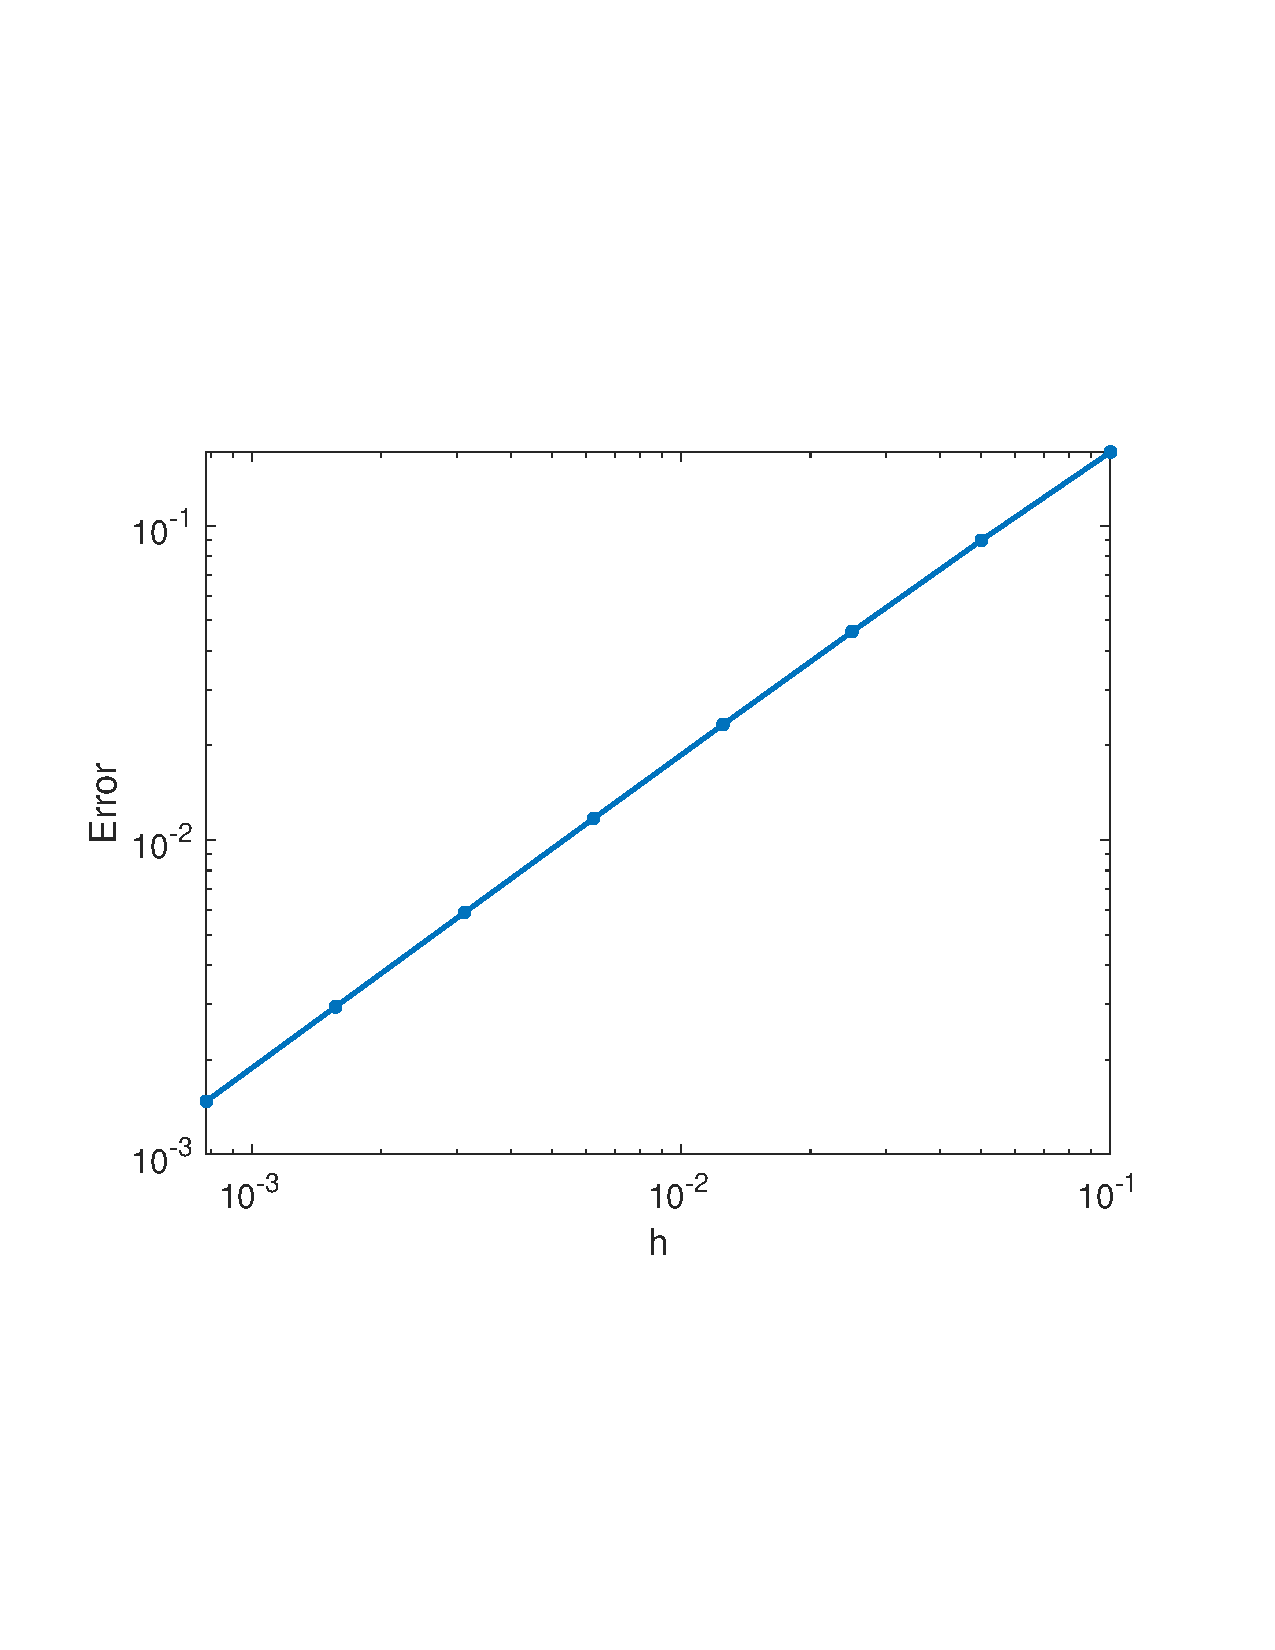
\includegraphics[height=6cm]{./figs/for_euler_conv}
    \end{equation*}
\begin{center}
$\Rightarrow \quad p$ appears to be $1$?
\end{center}
\end{itemize}
\end{frame}
%%%%%%%%%%%%%%%%%%%%%%%%%%%%%%%%%%%%%%%%%%%%
\begin{frame}{Numerical Experiment}{Results}
\begin{itemize}
    \item Calculate $p$ for successive values of $h$
        \[
        p \approx \frac{\log(e_{k}/e_{k-1})}{\log(h_k/h_{k-1})}
        \]

\begin{center}
\begin{tabular}{c|c|c|c|c|c}
Experiment $k$ & $e_k$ & $e_{k-1}$ & $h_{k}$ & $h_{k-1}$ &$p$\\ \hline 
 0& 0.1718& -& 1/10& - & -\\
 1& 0.08992& 0.1718& 1/20&  1/10&0.93 \\
 2&  0.04604& 0.08992& 1/40& 1/20&0.96\\
 3& 0.02330&  0.04604& 1/80& 1/40&0.98\\
 4& .01172& 0.02330& 1/160& 1/80&0.99 
\end{tabular}
\end{center}
\item $p \approx 1$
\question{
If the truncation error is $\mathcal{O}(h^2)$, then why is the numerical accuracy $\mathcal{O}(h)$?
}
\end{itemize}

\end{frame}
%%%%%%%%%%%%%%%%%%%%%%%%%%%%%%%%%%%%%%%%%%%%

\begin{frame}{Local and Global Error}
\begin{itemize}
    \item A local error starts from the \textbf{exact} value at $t_i$:
    \[
    \widehat{u}_{i+1}=u(t_i)+h f(t_i,u(t_i)).\]
    \[
    E_L=|u(t_{i+1})-\widehat{u}_{i+1}|=O(h^2).
    \]
    \item Global error compares the computed solution with the exact solution:
    \[E_G=|u(t_n)-\textbf{u}_n|.\]
    \item Intuition: $n=(b-a)/h$ steps each introduce an $O(h^2)$ error:
    \[ n\,O(h^2)=O(h). \]
\end{itemize}
\begin{block}{Euler's Global Error}
For a smooth solution and Lipschitz continuous $f$ in $u$, Euler's global error on a fixed interval is $O(h)$ as $h\to0$.
\end{block}
% Talking point: local error assumes an exact starting value. Global error
% also includes propagation of errors from previous steps; the sum is intuition.
\end{frame}

%%%%%%%%%%%%%%%%%%%%%%%%%%%%%%%%%%%%%%

\begin{frame}{Visualizing Local vs Global Error}
\begin{center}
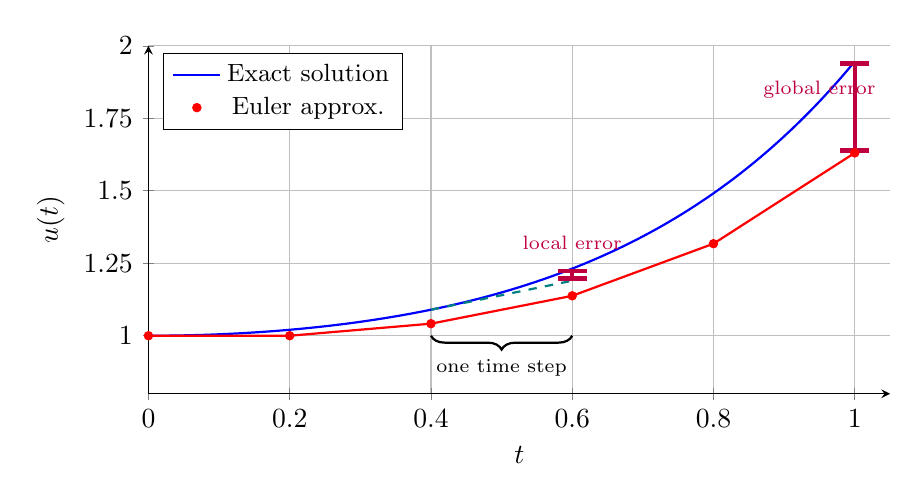
\begin{tikzpicture}
\begin{axis}[
    width=11cm,
    height=6cm,
    axis lines=left,
    xlabel={$t$},
    ylabel={$u(t)$},
    xmin=0, xmax=1.05,
    ymin=0.8, ymax=2.0,
    xtick={0,0.2,0.4,0.6,0.8,1.0},
    ytick={1,1.25,1.5,1.75,2.0},
    grid=both,
    legend style={at={(0.02,0.98)}, anchor=north west, font=\small},
    clip=false
]

% Exact solution
\addplot[
    domain=0:1,
    samples=200,
    thick,
    blue
] {3*exp(x^2/2) - x^2 - 2};
\addlegendentry{Exact solution}

% Euler approx points
\addplot[
    only marks,
    mark=*,
    mark size=1.5pt,
    red
] table[row sep=\\] {
x       y \\
0.0     1.0 \\
0.2     1.0 \\
0.4     1.0416 \\
0.6     1.1377 \\
0.8     1.3175 \\
1.0     1.6306 \\
};
\addlegendentry{Euler approx.}

% Euler line
\addplot[
    thick,
    red
] table[row sep=\\] {
x       y \\
0.0     1.0 \\
0.2     1.0 \\
0.4     1.0416 \\
0.6     1.1377 \\
0.8     1.3175 \\
1.0     1.6306 \\
};

% Local error: one Euler step from the EXACT value at t = 0.4
\addplot[dashed, thick, teal] coordinates {(0.4,{3*exp(0.4^2/2)-0.4^2-2}) (0.6,{(3*exp(0.4^2/2)-0.4^2-2)*1.08+0.0128})};
\addplot[|-|, ultra thick, purple] coordinates {(0.6, {(3*exp(0.4^2/2)-0.4^2-2)*1.08+0.0128}) (0.6, {3*exp(0.6^2/2) - 0.6^2 - 2})};
\node[align=left, font=\scriptsize, purple] at (axis cs:0.6,1.32) {local error};

% Local step indication brace
\draw [decorate,decoration={brace,mirror,amplitude=5pt}, thick]
  (axis cs:0.4,1) -- (axis cs:0.6,1) node[midway, below=5pt, font=\scriptsize] {one time step};

% Global error arrow at t = 1.0
\addplot[|-|, ultra thick, purple] coordinates {(1.0, 1.6306) (1.0, {3*exp(1^2/2) - 1^2 - 2})};
\node[align=left, font=\scriptsize, purple] at (axis cs:0.95,1.85) {global error};
\end{axis}
\end{tikzpicture}
\end{center}

\keyidea{

    \begin{itemize}
        \item The \textbf{local error} starts from the exact value for one step
        \item The \textbf{global error} accounts for all accumulated error
    \end{itemize}
}

\end{frame}

\sectionframe{Summary}

\begin{frame}{Differential Equations}
    \begin{itemize}
\item Differential equations describe how quantities change
\item Real-world problems $\rightarrow$ models $\rightarrow$ differential equations
\item Many useful differential equations lack a convenient closed-form solution
\end{itemize}

\vspace{3mm}

\keyidea{
We use numerical methods to approximate solutions.
}
\end{frame}

\begin{frame}{What Does a Computer Do?}

\begin{itemize}
\item We cannot compute the full function $u(t)$
\item Instead, we compute values at discrete times:
\[
t_0, t_1, t_2, \dots, t_n
\]
\item The entries of the numerical solution vector satisfy:
\[
\textbf{u}_i \approx u(t_i)
\]
\end{itemize}

\keyidea{
Continuous problem $\rightarrow$ discrete approximation
}

\end{frame}

\begin{frame}{Euler's Method}

\begin{itemize}
\item Based on Taylor expansion:
\[
u(t+h) \approx u(t) + h f(t,u)
\]
\item Update rule:
\[
\textbf{u}_{i+1} = \textbf{u}_i + h f(t_i, \textbf{u}_i)
\]
\end{itemize}

\keyidea{
Euler's method follows the slope (tangent line) step-by-step.
}

\end{frame}

\begin{frame}{Error in Euler's Method}

\begin{itemize}
\item Local error: (One step from an exact starting value)
\[
\mathcal{O}(h^2)
\]
\item Global error: (Accumulated error)
\[
\mathcal{O}(h)
\]
\end{itemize}

\vspace{3mm}

\keyidea{
Errors accumulate over many steps.
}

\end{frame}

\end{document}

